\documentclass[a4paper,11pt, twoside]{article}

\usepackage[a4paper,top=3cm,bottom=3.5cm,left=2.5cm,right=2.5cm]{geometry}
\usepackage{graphicx}
\usepackage[utf8x]{inputenc}
\usepackage[italian]{babel}
\usepackage{fancyhdr}
\usepackage{amssymb}
\usepackage{makeidx}
\usepackage{eurosym}
\usepackage{hyperref}
\usepackage{varioref}
\usepackage{xmpincl}
\usepackage{ccicons}
\usepackage{amsthm}

\theoremstyle{definition}
\newtheorem{defn}{Definizione}[section]

\title{Appunti di Automazione dei Sistemi Energetici}
\author{Matteo Gianello}
\date{\today}

\pdfinfo{%
  /Title    (Appunti di Automazione dei Sistemi Energetici)
  /Author   (Matteo Gianello)
  /Creator  (Matteo Gianello)
  /Producer ()
  /Subject  ()
  /Keywords (Automazione Sistemi Energetici Leva IngInf Polimi)
}

\includexmp{licenza}
\makeindex
\begin{document}
\pagestyle{empty}
\thispagestyle{empty}
\maketitle
\vspace{5cm}
\begin{center}
Quest'opera è stata rilasciata con licenza Creative Commons Attribuzione - Non commerciale - Condividi allo stesso modo 3.0 Unported. Per leggere una copia della licenza visita il sito web \url{http://creativecommons.org/licenses/by-nc-sa/3.0/deed.it} \ccbyncsa.
\end{center}
\newpage

\thispagestyle{plain}
\tableofcontents
\newpage

\pagestyle{plain}
\label{capitolo1}
\section{Introduzione}I sistemi che generano, distribuiscono e consumano energia sono diventati sempre pi� complessi ed articolati a causa di diversi tipi di sorgente dai quali l'energia viene ricavata (rinnovabili e non), diversi metodi di generazione, un mercato complesso ed in rapida evoluzione.\\
La progettazione di sistemi energetici richiede perci� sempre pi� la figura di un ingegnere automatico che abbia una visione del sistema a pi� livelli, permetta una sempre pi� alta integrazione e sia in grado di soddisfare le nuove esigenze.\\
Scopo del corso � quello di fornire una visione a livello di sistema dei problemi di controllo analizzando le soluzione adottate e gli sviluppi futuri senza entrare troppo nel dettaglio dei generatori e utilizzatori.
\subsection{L'automazione nei sistemi energetici}
I principi di automazione nei sistemi energetici li troviamo praticamente ovunque, nei refrigeratori, nelle caldaie, nelle lavatrici; pi� in generale nei generatori e nei consumatori.
A qualsiasi livello di progetto grandi componenti, macchinari industriali, piani energetici.\\
Praticamente l'automazione nei sistemi energetici � ovunque si abbia una trasformazione di energia, dove la parola "trasformazione" assume un significato diverso a seconda del contesto nel quale lavoriamo, ad esempio parliamo di "generazione" nel caso produzione di energia, "consumo" nel caso di utilizzo di energia e di "trasporto".\\
Ogni oggetto (o aggregazione di oggetti) pu� essere controllato per raggiungere degli obiettivi locali, ma bisogna sempre tener presente che ogni azione su un oggetto influenza l'intero sistema.\\
Nonostante tutto non si pu� definire una gerarchia tra i sistemi in quanto questa caratteristica richiederebbe un controllore enorme per eseguire il lavoro.\\
Possiamo comunque strutturare il sistema capendo quali sono i problemi rilevanti e se e come possono essere controllati ragionevolmente.
Un problema pu� essere dominato se la sua estensione � finita e pu� essere descritta da condizioni di confine specifiche ed � possibile trovare per esso almeno una soluzione di complessit� accettabile.\\
Per descrivere e capire il problema abbiomo bisogno di un approccio sistematico nel quale i componenti sono descritti a diversi livelli di dettaglio, preservano le loro interfacce con gli altri componenti e sono il pi� possibile indipendenti da come essi sono connessi con il resto del sistema.
\subsection{Definizioni di base}
Di seguito alcune definizione di base prima di cominciare.
\begin{description}
\item[Primary-Secondary energy(PE-SE)]:
\begin{itemize}
\item Primary Energy: � quell'energia che pu� essere ricavata direttamente in natura(gas, vento, sole);
\item Secondary Energy: � quell'energia ricavata trasformando l'energia primaria in una forma pi� facile da utilizzare, immagazzinare e trasportare.
\end{itemize}
\item[Renewable-Non Renewable Energy Sources (RES-NRES)]:
\begin{itemize}
\item Energia rinnovabile � ottenuta da una fonte di energia praticamente inesauribile.
\item Energia non rinnovabile richiede un consumo di "carburante" e il rilascio di inquinanti (es. petrolio, gas).
\end{itemize}
\item[Energy intensity]:Quantit� di energia per unit�; ad esempio per unit� prodotta o per servire una determinata richiesta.
\item[Energy conservation]: Riduzione in termini assoluti del consumo di energia.
\item[Energy efficenty]: Riduzione di EI preservando la quantit� di risultato.
\end{description}

\subsection{Alcuni problemi di controllo}
\begin{description}
\item[Controllo di generatori (PE$\rightarrow$ SE)]: minimizzare il consumo di carburante nel caso di NRES o massimizzare rendimento (RES).
\item[Controllo consumatori (SE$\rightarrow$fianl user)]:mantenere le condizioni ottimali (temperatura della stanza)
\end{description}

\label{capitolo2}
\section{Principi di modellazione}
I classici problemi di controllo sono divisi in "processi" e "motion" ma noi ci occuperemo principalmente dei primi. Incontreremo in oltre alcune PDE (Equazioni differenziali parziali) ma con al massimo una coordinata spaziale (tubi). In altri casi invece ci imbatteremo in sistemi di equazioni differenziali ordinarie ricavate dalla manipolazione di equazioni spaziali discrete ricavate da un approccio a volumi finiti (FV).\\
I tre aspetti principali dei quali ci occuperemo saranno sistemi di tipo idraulico, elettrico o termico; alcuni problemi di tipo meccanico si presenteranno ma solo sporadicamente e considereranno una sola coordinata spaziale.
\subsection{Sistemi termo-idraulici}
Le equazioni che incontreremo sono scritte facendo riferimento a un volume di controllo, non necessariamente costante, considerando un solo liquido incomprimibile.
\subsubsection{Equazione di bilancio delle masse}
L'equazione \ref{bmass} rappresenta l'equazione di bilancio delle masse dove $M$ è la massa di liquido contenuta nel volume di controllo, $w_i$ è il flusso che entra (se positivo) o esce (se negativo) dal volume di controllo.
\begin{equation}
\label{bmass}
\frac{dM(t)}{dt}=\sum_{i=1}^{n_m}w_i(t)
\end{equation}
\subsubsection{Equazione di bilancio dell'energia}
Le equazioni di bilancio dinamico che riguardano l'energia considerano un volume di controllo nel quale è contenuta tutta l'energia $E$ e dove $n_m$ flussi di massa e $n_h$ potenze termiche $Q_j$ entrano (escono se negativi).\\
Ovviamente la derivata dell'energia $E$ è la somma dei vari flussi termici ai quali non è associato alcun trasferimento di massa.\\
La derivata temporale dell'energia è data da due contributi coesistenti:
\begin{itemize}
\item apporti di energia legati al trasporto di massa dati da:
$$Portata \times Energia_-specifica_-del_-fluido$$
\item lavoro eseguito dal flusso entrante o uscente sul volume di liquido espresso in forma differenziale come:
$$dL=d(pv)=d(p/\rho)$$ o anche come $$dL=pdv+vdp$$
\end{itemize}
Dove la componente $pdv$ è detta "lavoro di compressione" e $vdp$ è il "lavoro di pulsione".
La grandezza che esprime l'apporto di energia di una portata di fluido entrante è data dalla \ref{entspec} che esprime l'entalpia specifica del fluido.
\begin{equation}
\label{entspec}
h=e+\frac{p}{\rho}
\end{equation}
Dove $e$ indica l'energia interna specifica.\\
Pertanto l'equazione di conservazione dell'energia è data dalla \ref{ener}
\begin{equation}
\label{ener}
\frac{dE(t)}{dt}=\sum_{i=1}^Nw_i(t)h_i(t)+\sum_{j=1}^MQ_j(t)
\end{equation}
Il termine $e$ domina (negli esempi ed esercizi di questo corso) di molto il termine $p/\rho$ in questo caso si può considerare l'entalpia e l'energia interna uguali e pari a $cT$ dove c è il calore specifico.
Detto ciò, tenendo conto delle nostre ipotesi e delle semplificazioni fatte, la formula del bilancio di energia si semplifica come nella \ref{bener}.
\begin{equation}
\label{bener}
c\frac{dM(t)T(t)}{dt}=c\sum_{i=1}^{n_m}w_i(t)T_i(t)+\sum_{j=1}^{n_h}Q_j(t)
\end{equation}
Alcune volte la massa rimane costante allora $$cM\frac{T(t)}{dt}=c\sum_{i=1}^{n_m}w_i(t)T_i(t)+\sum_{j=1}^{n_h}Q_j(t)$$
In altri casi è conveniente espandere la derivata a sinistra e sottrare l'equazione di massa moltiplicata per cT.
$$
\begin{array}{ccccccc}
cM(t)\frac{dT(t)}{dt} & + & cT(t)\frac{dM(t)}{dt} & = & c\sum_{i=1}^{n_m}w_i(t)T_i(t) & + & \sum_{j=1}^{n_h}Q_j(t)\\
\\
&-&cT(t)\frac{dM(t)}{dt}& = &-cT(t)\sum_{i=1}^{n_m}w_i(t)&&\\
\\
\hline
\\
cM(t)\frac{dT(t)}{dt}& + && = &c\sum_{i=1}^{n_m}w_i(t)(T_i(t)-T(t))&+&\sum_{j=1}^{n_h}Q_j(t)\\

\end{array}
$$
L'equazione precedente è chiamata equazione "net energy".\\
\subsubsection{Equazione della quantità di moto}
Per quanto riguarda la quantità di moto l'equazione in questo corso è utilizzata per modellizzare le condutture.\\
In un tubo la derivata della quantità di moto  è uguale alla somma delle forze che agiscono su di esso:
\begin{itemize}
\item pressione ai capi della conduttura
\item forza di gravità
\item forze di atrito sulle superfici laterali
\end{itemize}
tutte riferite lungo l'ascissa x del tubo (sull'asse y le componenti sono a 90° o sono bilanciate da forze esterne)
\begin{figure}
\centering
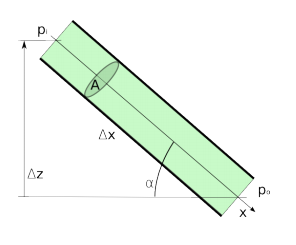
\includegraphics[width=5cm]{img/tubo.png}
\caption{Sezione di tubo\label{fig:tubo}}
\end{figure}
L'equazione dei momenti per il sistema in Fig. \ref{fig:tubo} è data dalla \ref{eqtubo} 
\begin{equation}
\label{eqtubo}
M\frac{du(t)}{dt}=A p_i(t)-A p_o(t)+ M g \sin(\alpha)-f_a(t)
\end{equation}
Dove $$f_a=K_f A_l\rho u|u|$$

La quantità $K_f$ è detta \emph{coefficente di frizione} e dipende dalle caratteristiche di contatto tra il fluido e le pareti. Inoltre la formula contiene un termine di inerzia che però nei nostri esempi non considereremo questo perchè i fenomeni idraulici sono molto più veloci delle costanti di tempo di quelli termici. Quindi la formula della quantità di moto si riduce alla \ref{qmoto}.
\begin{equation}
\label{qmoto}
A(p_i(t)-P_o(t))+Mg\frac{\Delta z}{\Delta x}-K_f A_l \rho u(t)|u(t)|=0
\end{equation}
Concludendo indicando con:
\begin{itemize}
\item A la sezione del tubo,
\item L la sua lunghezza
\item e $\omega $il suo perimetro interno
\end{itemize}
e ricordando che $w=\rho A u$ abbiamo che:
$$p_i-p_o= K_f\frac{\omega L}{\rho A^3} w|W|-\rho g\Delta z$$
L'equazione della quantità di moto può rappresentare il comportamento tipico di una valvola. Dal nostro punto di vista una valvola è come una piccola sezione variabile di tubo in cui $\Delta z =0$ e la velocità è data dalla formula seguente:
$$w=C_v\phi(x)\sqrt{\rho (p_i - p_o)}$$
dove $C_v$ è il coefficente di flusso e $\phi(x)$ è la caratteristica intrinseca della valvola.
\subsubsection{Equazione dell'energia nei corpi solidi}
Per quanto riguarda il caso in cui non vi sia scambio di massa (ad esempio conduzzione attraverso una parete) la formula diventa:
$$cM\frac{dT(t)}{dt}=\sum_{j=1}^{n_h}Q_j(t)$$
Nel caso in cui il muro non sia uniforme lo si divide in più livelli e si applica sempre la stessa formula.\\
\subsubsection{Equazioni dei flussi di calore}
Le equazioni per i flussi di calore ci servono per modellizzare tre fenomeni:
\begin{itemize}
\item Conduzione
\item Convezione
\item Irraggiamento
\end{itemize}
Per quanto riguarda la conduzione la potenza termica è data da :
$$Q_{ab}=G(T_a(t)-T_b(t))$$
Dove $T_a$ e $T_b$ sono le temperature ai due lati e G è:
$$G=\lambda \frac{A}{s}$$
con A la superfice s lo spessore e $\lambda$ la conduttività termica del materiale.\\
Nel caso di convezione la formula della potenza termica tra flusso e parete è data da:
$$Q_{wf}=\gamma A(T_w(t)-T_f(t))$$
\subsection{Sistemi elettrici}
Per quanto riguarda i sistemi elettrici saranno effettuate alcune semplificazioni per rendere più chiari ed intuitivi i concetti:
\begin{itemize}
\item una sola sincrona frequenza per tutta la rete.
\item tutti i generatori forniranno un voltaggio costante.
\item le linee di trasmissione avranno un comportamento lineare.
\item sistemi ad una fase
\end{itemize}
Inoltre adotteremo un sistema di modellizzazione basato sui fasori.\\
Ogni quantità che varia in modo sinusoidale a frequenza costante $\omega$ può essere rappresentata come segue:
$$A\cos(\omega t +\theta)= \Re(Ae^{j(\omega t+\theta)})=\Re(Ae^{j\theta}e^{j\omega t})$$
Dove il fasore $A^{j\theta}$ esprime la fase e l'ampiezza rispetto a un opportuno sistema di riferimento.
\subsubsection{La legge di Ohm}
$$\underline{V}=\underline{Z}\underline{I},\underline{I}=\underline{Y}\underline{V}$$
dove $\underline{V},\underline{I}$ sono rispettivamente i fasori che indicano voltaggio e corrente e $\underline{Z},\underline{Y}$ sono impedenza e ammettenza. Tipicamente le ultime due quantità vengono espresse come $\underline{Z}=R+iX$ e $\underline{Y}=G-iB$ dove $R,X,G,B$ sono rispettivamente la resistenza, la reattanza, la conduttanza e la suscettanza.\\
La potenza espressa in termini di fasori è data da:
$$S=V_{RMS}I^*_{RMS}=P+jQ=Ae^{j\phi}$$
dove possiamo distinguere una componente attiva:
$$P=\Re(S)=V_{RMS}I_{RMS}\cos \phi$$
e una componente reattiva:
$$Q=\Im(S)=V_{RMS}I_{RMS}\sin \phi$$

\label{capitolo3}
\section{Modelli a blocchi e ad oggetti}
Per identificare dei modelli o dei parametri a volte ci affidiamo a delle simulazioni di modelli che possono essere di due tipi:
\begin{itemize}
\item Orientati ai blocchi
\item Orientati agli oggetti
\end{itemize}
Nel caso di modelli orientati ai blocchi l'ordinamento è di tipo \emph{causale} ovvero un blocco ha un ingresso ed un uscita e un uscita può connettersi a uno o più ingressi attraverso connessioni \emph{input/output}.
Nel caso di modelli orientati agli oggetti abbiamo una \emph{a-causalità} tra i vari oggetti; le connessioni tra i vari oggetti avvengono attraverso delle porte che instaurano un collegamento di uguaglianza tra ciò che viene collegato.
Vediamo ora attraverso un esempio la differenza tra modelli BO e OO.
\subsection{Legge di Ohm}
\subsubsection{Caso BO}
Se voglio modellizzare un resistore collegato ad un generatore dovrò costruire due modelli, uno nel caso in cui il generatore è un generatore di tensione, in questo caso il modello è dato da:
$$
\begin{array}{ccc}
V&=&E\\
I&=&V/R
\end{array}
$$
Nel caso in cui invece il generatore fornisca una corrente il modello diventa:
$$
\begin{array}{ccc}
I&=&A\\
V&=&RI
\end{array}
$$
Per gli stessi componenti abbiamo dovuto definire due differenti condizioni limite e \emph{due modelli differenti}.
\subsubsection{Caso OO}
Nel caso di modelli orientati agli oggetti opto per un differente approccio; prima di tutto diamo una definizione di \emph{porte}: esse possono essere definite come quei terminali fisici che interfacciano il componente con il mondo esterno. Nel caso del resistore sono i due pin di connessione. Il modello del resistore diventa quello identificato nell'equazione \ref{res}
\begin{equation}
\label{res}
RES:
\left\{
\begin{array}{ccc}
a.I+b.I&=&0\\
a.V-b.V&=&R a.I
\end{array}
\right .
\end{equation}
Introduciamo poi i due generatori rispettivamente quello di tensione \ref{vgen} e quello di corrente \ref{cgen} ed inoltre la massa \ref{gnd}
\begin{equation}
\label{vgen}
VGEN:
\left\{
\begin{array}{ccc}
a.I+b.I&=&0\\
a.V-b.V&=&R E
\end{array}
\right.
\end{equation}
\begin{equation}
\label{cgen}
CGEN:
\left\{
\begin{array}{ccc}
a.I+b.I&=&0\\
a.I&=&-A
\end{array}
\right.
\end{equation}
\begin{equation}
\label{gnd}
GND:\quad a.V=0
\end{equation}
\begin{figure}
\centering
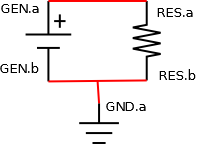
\includegraphics[width=5cm]{img/circuito.png}
\caption{Schema del circuito in rosso le connessioni\label{fig:circuito}}
\end{figure}
Cosi facendo vediamo come i due modelli descritti prima attraverso il sistema BO in questo caso possano essere descritti semplicemente cambiano il \emph{"modulo"} generatore; ovvero interscambiando le equazioni che descrivono i due generatori.\\
Bisogna però descrivere le equazioni che governano le connessioni (Fig. \ref{fig:circuito}), che anche in questo caso sono comuni per i due tipi di generatori.\\
\begin{eqnarray}
GEN.a.V &=& RES.a.V\\
GEN.a.I + RES.a.I &=& 0\\
GEN.b.V &=& GND.a.V\\
RES.b.V &=& GND.a.V\\
GEN.b.I + RES.b.I + GND.a.I &=& 0
\end{eqnarray}
Le variabili che caratterizzano una porta possono essere di due tipi:
\begin{itemize}
\item variabili di \emph{effort} ovvero variabili che sono definite attraverso la differenza da un riferimento (es. ddp).
\item variabili \emph{flow} definite come un flusso attraverso un canale (es. corrente).
\end{itemize}
Per connettere N porte ho bisogno di $N-1$ equazioni per ogni variabile di effort ed una sola per tutte le variabili di flusso.\\
Come si è visto entrambi i metodi di modellizzazione incapsulano il comportamento del modello esponendo un'interfaccia, questo per ragioni di scalabilità. I modelli BO richiedono però che il sistema sia orientato cioè richiede che le variabili di ingresso e uscita siano ben specificate per ogni blocco. Nei modelli OO, invece, non è richiesto che i componenti siano orientati.

\subsection{Concetto di circuito elettrico equivalente}
Nei modelli OO le porte sono naturalmente associate ad un trasferimento di energia. Ad esempio consideriamo una porta con un unica variabile di flusso e una di effort in diversi casi:
\begin{itemize}
\item elettrico (tensione v e corrente i): vi = potenza
\item meccanico translazionale (posizione x e forza f): $\dot{x}$f = potenza
\item meccanico rotazionale (angolo $\theta$ fozta $\tau$): $\dot{\theta}\tau$ = potenza
\item termico (temperatura T e potenza Q): in questo caso la potenza non è il prodotto delle due
\end{itemize}
L'equivalente elettrico è utile anche per descrivere quei fenomeni legati all'energia; come nel caso in cui:
\begin{itemize}
\item l'accumulo di energia è legato a una variabile di effort come nel caso $E=CT$ dove $C$ è la capacità termica.
\item il trasferimento di energia è legato linearmente a una differenza di variabili $Q=G\Delta T$ dove $G$ è la conduttanza termica.
\end{itemize}

\label{capitolo4}
\section{Modelli e problemi di controllo}
Nel controllo di sistemi elettrici possiamo incontrare due tipi di problemi:
\begin{itemize}
\item \textbf{problemi di controllo di potenza} nei quali si cerca di fornire la potenza richiesta agli utilizzatori; minimizzando i costi globalmente o fornendo la massima potenza richiesta minimizzando i costi del singolo generatore.
\item \textbf{problemi di controllo di energia} nei quali si richiede che l'elettricità abbia voltaggio e frequenza necessari per cooperare con tutti i generatori e i carichi. 
\end{itemize}
Questi problemi sono apparentemente interlacciati in quanto dipendono entrambi dai generatori. Inoltre, solo ai generatori si applicano i meccanismi di controllo mentre i carichi sono considerati disturbi esogeni.\\
Possiamo considerare due tipi di generatori, il primo con masse rotanti e alternatori, il secondo senza masse rotanti ma con inverter.
I generatori con masse rotanti forniscono la potenza richiesta aumentando o diminuedo la velocità di rotazione con conseguente alterazione della frequenza.\\
Quando ci spostiamo dal controllo dei generatori al controllo del carico della rete incontriamo un secondo problema ovvero il problema del flusso di carico; infatti si vuole distribuire la potenza senza però sovraccaricare le linee e possibilmente minimizzando le perdite di carico.\\
\subsection{Modello di un generatore termoelettrico}
Questo tipo di generatore è formato da una massa rotante nel quale potenza e frequenza sono accoppiate.\\
Prendiamo il caso di un generatore isolato nel quale abbiamo una fornace nella quale si brucia del carburante e di conseguenza si produce calore, il calore prodotto trasforma un fluido in vapore, questo vapore fa muovere una turbina che infine fa muovere l'alternatore.\\
Prendiamo in considerazione come ingresso il sistema che brucia carburante e come uscita la potenza meccanica dell'alternatore. Per semplicità consideriamo come ingresso esogeno la potenza $P_c$ prodotta dalla combustione e rilasciata al contenitore principale di energia (vapore).
Il bilancio di energia immagazzinata è dato da:
$$\dot{E}= P_c-P_{loss}-P_t$$
dove $P_{loss}$ è la potenza persa nelle pareti esterne mentre $P_t$ è la potenza consumata dalla turbina.
Per semplicità assumiamo che l'immagazzinatore di energia sia completamente vapore e che la sua massa sia costante; a questo punto possiamo associare la $P_{loss}$ alla differenza di temperatura tra la temperatura di saturazione del vapore a una certa pressione $p$ e la temperatura esterna tramite la relazione:
$$P_{lost}=G_{loss}(T_{sat}(p)-T_{ext})$$
In generale la $T_{sat}>>T_{ext}$ così possiamo scrivere che:
$$P_{loss}=K_{loss}\frac{E}{M}$$
dove $K_{loss}$ è un opportuno parametro legato alla superficie di dispersione, e la divisione per $M$ esprime la dipendenza della potenza dallo stato del vapore.\\
Un'altra semplificazione riguarda $P_t$ infatti trascuriamo il surriscaldamento che subisce il vapore all'atto dell'attraversamento della turbina e facciamo dipendere $P_t$ soltanto dalla pressione ($E/M$) e dall'apertura della valvola della turbina $\theta \in [0,1]$
$$P_t=\theta K_{draw} \frac{E}{M}$$
e dove $K_{draw}$ è un altro parametro.\\
La potenza meccanica che raggiunge l'alternatore è ottenuta tenendo conto dell'efficenza meccanica dell'alternatore assunta costante e chiamata $\eta_m$
$$P_m=\eta_m P_t$$
Mettendo le equazioni a sistema otteniamo
\begin{equation}
\left\{
\begin{array}{ccccc}
\dot{E}&=&P_c-K_{loss}E/M&-&\theta K_{draw}E/M\\
\\
P_m&=&\eta_m\theta K_{draw}E/M&&
\end{array}
\right.
\end{equation}
Sapendo che $[K_{loss}E/M]=[K_{draw}E/M]=[W]$ e $\theta$ e $\eta_m$ sono adimensionali ricaviamo che $[K_{loss}/M]=[K_{draw}/M]=[1/s]$ e possiamo riscrivere il sistema precedente come:
\begin{equation}
\left\{
\begin{array}{ccccc}
\dot{E}&=&P_c-\big(\frac{1}{T_{loss}}&+&\frac{\theta}{T_{draw}}\big)E\\
\\
P_m&=&\frac{\eta_m}{T_{draw}}E\theta &&
\end{array}
\right.
\end{equation}
In questo caso $T_{loss}$ e $T_{draw}$ sono le costanti di tempo con le quali l'energia viene rispettivamente persa dalla superficie esterna e prodotta attraverso l'alternatore alla massima apertura della valvola della turbina.
Questo modello risulta molto impreciso e in un caso reale sarebbe applicabile solo nell'intorno di un punto di lavoro. Ma per i nostri scopi è più che sufficente.\\
Introduciamo ora la potenza nominale del generatore $P_n$ e chiamiamo $T_{rest}$ il tempo richiesto dal generatore per immagazzinare la sua "energia nominale" definita come $E_n=P_nT_{rest}$. Dividiamo ora entrambe le equazioni per $E_n$
\begin{equation}
\left\{
\begin{array}{ccccccc}
\dot{e}&=&\frac{1}{T_{rest}}p_c&-&\big(\frac{1}{T_{loss}}&+&\frac{\theta}{T_{draw}}\big)e\\
\\
p_m&=&\eta_m\frac{T_{rest}}{T_{draw}}e\theta&&&&
\end{array}
\right.
\end{equation}
Dove $p_c=P_c/P_n$ e $p_m= P_m/P_n$ sono rispettivamente la potenza normalizzata di combustione e meccanica, ed $e=E/E_n$ è l'energia normalizzata.\\
A questo punto calcoliamo l'equilibrio di questo modello per ingressi costanti $\overline{p_c},\overline{\theta}$
$$\overline{e}=\frac{T_{draw}T_{loss}\overline{p_c}}{T_{ress}(T_{draw}+T_{loss}\overline{theta})}$$
$$\overline{p_m}=\frac{\eta_mT_{loss}\overline{p_c}\overline{\theta}}{T_{draw}+T_{loss}\overline{\theta}}$$
A questo punto linearizziamo il modello nelle vicinanze dell'equilibrio imponendo $\Delta p=p_c-\overline{p_c}, \Delta\theta=\theta-\overline{\theta}$ e $\Delta e = e- \overline{e}, \Delta p_m =p_m-\overline{p_m}$
$$
\left\{
\begin{array}{ccccc}
\Delta\dot{e}&=&-\left(\frac{1}{T_{loss}}+\frac{\overline{\theta}}{T_{draw}}\right)\Delta e&+&\left[\frac{p_c T_{loss}}{T_{rest}(T_{draw}+T_{loss}\overline{\theta})}\frac{1}{T_{rest}}\right]\left[\begin{array}
{c}
\Delta\theta\\
\Delta p_c
\end{array}\right]\\
\\
\left[
\begin{array}{c}
\Delta p_m\\
\Delta e
\end{array}\right] 
& = &
\left[
\begin{array}{c}
\frac{\eta_mT_{rest}\theta}{T_{draw}}\\
1
\end{array}\right]
\Delta e &+&
\left[ 
\begin{array}{cc}
\frac{\eta_mT_{loss}\overline{p_c}}{T_{draw}+T_{loss}\overline{\theta}} & 0 \\
0 & 0
\end{array}\right]\left[
\begin{array}{c}
\Delta\theta\\
\Delta p_c
\end{array}\right]
\end{array}
\right.
$$
La corrispondente matrice di trasferimento è:
$$
\begin{array}{lc}
\Gamma(s) &=\left[\begin{array}{cc}
\Gamma_{\theta_m}(s) & \Gamma_{c_m}(s)\\
\Gamma_{\theta_e}(s) & \Gamma_{c_e}(s)
\end{array}\right]=\left[\begin{array}{cc}
\frac{\Delta p_m(s)}{\Delta\theta(s)} & \frac{\Delta p_m(s)}{\Delta p_c(s)}\\
\frac{\Delta e(s)}{\Delta\theta(s)} & \frac{\Delta e(s)}{\Delta p_c(s)}
\end{array}\right]\\
\\
\dots &= \frac{1}{1+s\frac{T_{draw}T_{loss}}{T_{draw}+T_{loss}\overline{\theta}}}
\left[
\begin{array}{cc}
\frac{\eta_m T_{draw}T_{loss}\overline{p_c}}{(T_{draw}+T_{loss}\overline{\theta})^2}(1+sT_{loss})&
\frac{\eta_mT_{loss}\overline{\theta}}{T_{draw}+T_{loss}\overline{\theta}}\\
\frac{T_{draw}T^2_{loss}\overline{p_c}}{T_{rest}(T_{draw}+T_{loss}\overline{\theta})^2} & 
\frac{T_{draw}T_{loss}}{T_{rest}(T_{draw}+T_{loss}\overline{\theta})}\\
\end{array}
\right]
\end{array}
$$
Alcune altre semplificazioni che faremo a livello di sistema per valutare i costi sono:
\begin{itemize}
\item Assumeremo che i costi siano dati solo dal consumo di carburante e non dal mantenimento dell'impianto
\item La combustione non avviene allo stesso modo ai diversi carichi di sistema
\item Il cunsumo specifico $c_s$è definito tipicamente decrescente rispetto a $P_c$.
\item Il flusso di carburante consumato $w_c$ e $p_c$ sono legati dall'equazione
$$w_c=c_s(p_cP_n)p_cP_n;$$
\end{itemize}
La potenza attiva richiesta dal carico, un parametro esogeno per il generatore, viene detta $P_e$ così il bilancio delle energie per la massa in rotazione è:
$$J\omega\dot{\omega}=P_m-P_e$$
dove $J$ è l'inerzia totale vista all'albero del generatore (si pensi al caso di più generatori).
L'equazione del rendimento all'equilibrio  per ogni $\omega$ e $\overline{P_m}$ e $\overline{P_e}$ siano costanti e coincidenti la linearizazione diventa:
$$\Delta\dot{\omega}=-\frac{P_m-P_e}{J\overline{\omega}^2}\Delta\omega+\frac{1}{J\overline{\omega}}(\Delta P_m-\Delta P_e)$$
Visto che $P_e=P_m$ e che $\omega$ viene regolato al valore desiderato $\omega_0$ otteniamo:
$$\Delta\dot{\omega}=\frac{1}{J\omega_0}(\Delta P_m-\Delta P_e)$$
Normalizzando $P_{m,e}$ con $P_n$ e $\omega$ con $\omega_0$ e usando $\delta$ per indicare le variazioni delle quantità normalizzate otteniamo:
$$\frac{\Delta\dot{\omega}}{\omega_0P_n}=\frac{1}{J\omega_0}(\frac{\Delta P_m}{\omega_0P_n}-\frac{\Delta P_e}{\omega_0P_n})$$
$$\delta\dot{\omega}=\frac{1}{J\omega_0^2}(\delta P_m-\delta P_e)$$

\subsection{Controllo di un generatore}
Dopo aver descritto la relazione che lega $(\Delta\omega, \Delta p_c)\rightarrow(\Delta p_m, \Delta e)$ e la matrice di trasferimento del primo ordine $\Gamma (s)$. Ricordando inoltre che il contenuto di energia è legato alla pressione del vapore $p$.
Ora parleremo del controllo di pressione nel generatore che significa anche controllare l'energia contenuta nel generatore.\\
Per effettuare questo controllo il nostro problema diventa come controllare la potenza meccanica in uscita dall'alternatore. Per applicare questo controllo si utilizzano principalmente tre metodi:
\begin{itemize}
\item \textbf{boiler follows}: consiste nella modulazione di $\theta$ oer modulare $\Delta P_m$ e $\Delta P_c$ per mantenere costante la pressione; questo permette una regolazione di $P_m$ molto rapida ma che provoca piccole variazioni di pressione che causano un forte stress al sistema.
\item \textbf{turbine follows} consiste nell'usare $\omega$ e $P_c$ per regolare il sistema; con questo metodo si ha un controllo sulla pressione migliore ma il tempo di risposta del sistema è più lento.
\item \textbf{sliding pressure} In questo sistema si mantiene $\theta$ al suo valore massimo e si controlla $P_m$ agendo su $w_c$; questo sistema permette di non sollecitare troppo la turbina ma come contro ha dei tempi di risposta molto lunghi.

\end{itemize}

Descriviamo ora gli attuatori che controllano $\theta$ e $P_c$ tenendo conto dei loro tempi di risposta che non sono sicuramente immediati. La matrice di trasferimento è:
$$A(s)=\left[\begin{array}{cc}
\frac{1}{1+sT_{\theta}} & 0\\
\\
0 & \frac{1}{1+sT_{P_c}}\\
\end{array}\right]$$
Quindi in accordo con le dinamiche degli attuatori:
$$\left[\begin{array}{c}
\Delta\theta(s)\\
\Delta P_c(s)
\end{array}\right]=A(s)\left[\begin{array}{c}
\Delta\theta_c(s)\\
\Delta P_{cc}(s)
\end{array}\right]$$
Dove $\theta_c$ e $P_{cc}$ sono le variabili di comando degli attuatori rispettivamente di $\theta$ e $P_c$
Il sistema è così modellizzato dalla matrice di trasferimento $\Gamma(s)A(s)$\\
D'ora in poi non indicheremo più il pedice "c" per indicare le variabili di controllo e considereremo A(s) come parte del processo, ovvero considerando sempre la cascata tra $A$ e $\Gamma$ ma prendendo come ingressi $\theta$ e $P_c$. In altre parole possiamo scrivere il sistema come:
$$
\left[\begin{array}{c}
\Delta P_m(s)\\ \Delta e(s)
\end{array}\right] 
= \Gamma_{ap}(s)
\left[\begin{array}{c}
\Delta\theta(s)\\ \Delta P_c(s)
\end{array}\right]
$$
dove $\Gamma_{ap}(s)=\Gamma(s)A(s)$\\

Tornando allo scopo principale, il tipo di politica di controllo utilizzata per controllare il sistema si basa su quali tipi di generatori vengono utilizzati, sulle regole della rete e talvolta anche in base al carico presente in quell'istante.
Qualsiasi sia la politica di controllo scelta e qualsiasi sia la variabile di controllo usata per governare $P_m$ (d'ora in poi denotata con $u_P$) il sistema può essere controllato dalla funzione di trasferimento $G(s)$ espressa come:
$$G(s)= \frac{\Delta P_m(s)}{\Delta u_P(s)}\Bigg|_{struttura_-generatore,politica_-di_- controllo}$$

Possiamo normalizzare $G(s)$ sostituendo la potenza normalizzata $P_n$ e la variabile di controllo normalizzata $u_{P_n}$ ottenendo:
$$g(s)=\frac{\delta P_m(s)}{\delta u_p(s)}$$
dove $u_{P_n}$ è 1 o $P_n$ se la variabile di controllo è rispettivamente o $\theta$ o $P_c$ in ogni caso lo schema da controllare risulta essere (per un generatore isolato):
\begin{figure}[htb]
\centering
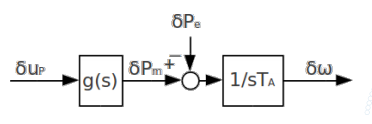
\includegraphics[width=10cm]{img/geniso.png}
\caption{Schema a blocchi di un generatore isolato}
\label{fig:geniso}
\end{figure}
Per il caso di generatore isolato il sistema di controllo risulta essere quello in figura \ref{fig:gencontrol}
\begin{figure}[htb]
\centering
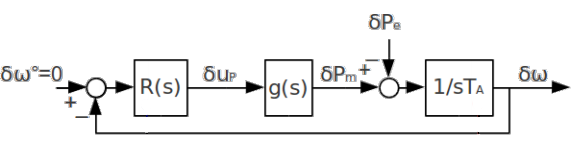
\includegraphics[width=10cm]{img/gencontrol.png}
\caption{Schema del sistema di controllo per un generatore isolato}
\label{fig:gencontrol}
\end{figure}
Dove $1/sT_A$ è un integratore che impone a zero l'uscita in caso di sistema all'equilibrio, mentre $R(s)$ è un altro integratore per mantenere a zero l'errore di frequnza nel caso di sistema all'equilibrio.
\subsection{Generatori in rete}
Prima di parlare del caso di più generatori connessi in rete dobbiamo fare alcune ipotesi sulla rete stessa; infatti si suppone che la rete sia rigida e sincrona. I generatori invece ruotano alla stessa velocità senza drift sul valore impostato.
In questo caso tutta la potenza meccanica (non normalizzata) viene sommata, mentre un unica potenza elettrica viene sottratta (il totale del carico). Il sistema sotto controllo è rappresentato in figura \ref{fig:gennetwork}
\begin{figure}[htb]
\centering
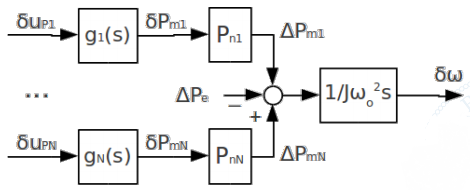
\includegraphics[width=10cm]{img/gennetwork.png}
\caption{Sistema di più generatori collegati alla 
rete.}
\label{fig:gennetwork}
\end{figure}
Dove $J$ è l'inerzia totale della rete.\\
A questo punto è facile estendere lo schema del generatore isolato allo scema con più generatori come vediamo in figura \ref{fig:netcontrol}.
\begin{figure}[htb]
\centering
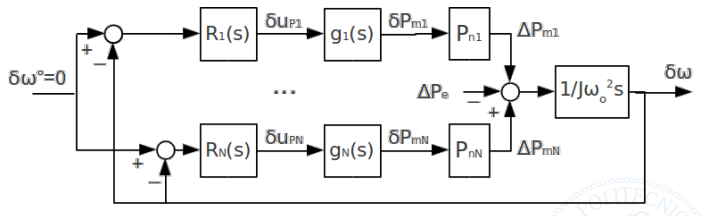
\includegraphics[width=10cm]{img/netcontrol.png}
\caption{Schema del sistema di controllo per un generatore isolato}
\label{fig:netcontrol}
\end{figure}
In questo schema l'integratore ($1/J\omega_0^2s$) garantisce che l'errore sulla potenza in caso di equilibrio sia zero. Mentre i regolatori ($R_1\dots R_n$) non possono essere tutti degli integratori altrimenti avremo delle parti non controllabili del sistema.\\
Per capire il perchè osserviamo lo schema di figura \ref{fig:schema} equivalente al sistema.
\begin{figure}[htb]
\centering
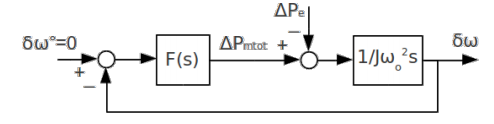
\includegraphics[width=10cm]{img/schema.png}
\caption{Schema equivalente}
\label{fig:schema}
\end{figure} 
Dove $\Delta P_{mtot}$ è la variazione della potenza meccanica totale, e
$$F(s)=\sum_{i=1}^N R_i(s)g_i(s)P_{ni}$$
Degli integratori in $R_i$ andrebbero in parallelo e farebbero perdere la controllabilità.\\
La soluzione a questo problema è avere un solo integratore:
\begin{itemize}
\item avere un primo regolatore $R_i(s)$ di tipo proporzionale.
\item introdurre un controllore in seconda frequenza di tipo integrale per l'intera rete.
\item l'output del secondo regolatore entra in alcuni correttori che entrano a loro volta nell'ingresso degli $R_i$
\end{itemize}
\section{Applicazione del paradigma OO al modello del generatore}
Fino ad ora abbiamo utilizzato un approccio orientato ai blocchi per descrivere il nostro sistema; ora però diviene più utile descrivere tale sistema con un modello orientato agli oggetti.\\
A questo scopo, come prima cosa definiamo un connettore che esprima l'accoppiamento sincrono e rigido, ovvero nel quale tutti i modelli connessi hanno la stessa frequenza e non presentano fenomeni di disallineamento.
\begin{verbatim}
connector PowerFreqPort
		  Real f; // Frequency
	flow Real P; // Power
end PowerFreqPort;
\end{verbatim}
Definiamo una rete nella quale potremmo collegare diversi generatori ma che controlla una singola inerzia globale.
\begin{verbatim}
model ElectricNetworkPF
	signalIn Pe; // Electric power (exogenous)
	PowerFreqPort Pg; // Port to connect all generators
	parameter Real J = 1000; // Inertia
	parameter Real fo = 50; // Nominal (and initial) frequency
	Real f(start = fo); // Frequency
equation
	der(f) = (Pg.P-Pe)/(J*8*3.14^3*fo^2); // der(2*pi*f)=(Pg-Pe)/(J*(2*pi*fo)^2)
	f = Pg.f;
end ElectricNetworkPF;
\end{verbatim}
Ed infine definiamo il modello del generatore:
\begin{verbatim}
model SimpleThermoElecGenPF
	signalIn 		theta; // Throttling valve command
	signalIn 		Pc; // Combustion power command
	PowerFreqPort  Pg; // Port to network
	parameter Real Pn = 100;
	parameter Real Trest = 500;
	parameter Real Tdraw = 500;
	parameter Real Tloss = 1e9;
	parameter Real etam = 0.95;
	parameter Real thetabar = 0.8;
	parameter Real pcbar = 0.8;
	Real e(start=Tdraw*Tloss*pcbar/Trest/(Tdraw+Tloss*thetabar));
	Real pc,pm;
equation
	der(e) = pc/Trest-(1/Tloss+theta/Tdraw)*e;
	pm = etam*e*theta;
	pc = Pc/Pn;
	pm = Pg.P/Pn;
end SimpleThermoElecGenPF;
\end{verbatim}

\label{capitolo5}
\section{Ottimizzazione dei costi di generazione}
Consideriamo una rete con $N$ generatori nella quale in ogni istante la potenza meccanica totale è uguale alla potenza elettrica richiesta.
$$\sum_{i=1}^{N}P_{mi}= P_e$$
Il controllo primario e secondario assicurano questa condizione ed inoltre mantengono la frequenza costante ad un certo setpoint. Ora ci chiediamo però qual'è il costo di tale operazione; conoscendo la curva di efficenza di ogni generatore possiamo scrivere N equazioni che relazioni le $P_{gi}$ (potenza generata dal generatore i) ad un \emph{cost rate} $c_i[\EUR/s]$. Possiamo esprimere tale relazione come $c_i(P_{gi})$ che è una funzione monotona crescente nel quale $P_{gi}$ può variare tra un valore massimo e un valore minimo $P_{gi,min}\leq P_{gi}\leq P_{gi,max}$.\\
Il problema che ci poniamo ora è quello di minimizzare il costo, o più semplicemente minimizzare il cost rate totale.
$$
\begin{array}{cc}
min &\sum_{i=1}^N c_i(P_{gi})\\
\\
s.t. &\sum_{i=1}^NP_{gi}=P_e\\
\\
&P_{gi,min}\leq P_{gi}\leq P_{gi,max} \quad i=1\dots N
\end{array}
$$
Sarebbe risultato più complicato trovare il valore ottimo di cost rate per il singolo generatore ma questa soluzione permette di capirne il funzionamento con un buon compromesso sull'ottimalità della soluzione finale.\\
Molto frequentemente il modello di costo viene rappresentato come un polinomio di terzo grado del tipo:
$$c_i(P_{gi})=(k_{g1}P_{gi}+k_{g2}P_{gi}^2+k_{g3}P_{gi}^3)k_F+k_{om0}+k_{om1}P_{gi}$$
Dove $k_{gj}$ è il coefficente di costo per la produzione di energia, $k_F$ è il costo del carburante per unità di energia e $k_{om\textit{l}}$ è il costo di mantenimento dell'impianto.\\
Il motivo per qui si tende ad utilizzare un polinomio di ordine 3 è il fatto che il \emph{power ratio} $r_{fP}(P_g)=Q_f(P_g)/P_g$, dove $Q_f$ è la potenza generata dal carburante e $P_g$ è la potenza generata dal generatore e considerando che la quantità $r_{fP}$ è adimensionale, abbia un minimo nel punto di ottimo. Il modo migliore per sintetizzare il modello è quello di descrivere la funzione $r_{fP}(P_g)$ come una parabola con un punto di ottimo nel vertice $r_{fP}^o$, la frazione $p_g^o$ di $ P_{g,max}$ corrisponde al rapporto ottimo dove la funzione $p_g$ è definita come $P_g/P_{g,max}$, ed infine il massimo power ratio $r_{fP}^{ml}$ al minimo carico sostenibile 	$p_g^{ml}= P_{g,min} /P_{g,max}$
Così da ottenere 
$$
r_{fP}(p_g)= r_{fP}^o+\frac{r_{fP}^{ml}-r_{fP}^o}{(p_g^o-P_g^{ml})^2}+(p_g-p_{g}^o)^2;
$$
e
$$
r_{fP}(P_g)= r_{fP}^o+\frac{r_{fP}^{ml}-r_{fP}^o}{(P_g^o-P_{g,min})^2}+(P_g-P_{g}^o)^2;
$$
A questo punto possiamo scrivere 
$$
Q_f(P_g)=r_{fP}P_g=\left (r_{fP}^0\frac{r_{fP}^{ml}-r_{fP}^o}{(P_g^o-P_{g,min})^2}+(P_g-P_{g}^o)^2\right ) P_g
$$
Che contiene le potenze d $P_g$ dalla 1 alla 3 così possiamo scriverlo come $k_{g1}P_{gi}+k_{g2}P_{gi}^2+k_{g3}P_{gi}^3$ ed in particolare abbiamo che:
$$
k_{g1}=\frac{r_{fP}^{ml}{P^o_g}^2-r_{fP}^oP_{g,min}(2P^o_g-P_{g,min})}{(P^o_g-P_{g,min})^2}
$$
$$
k_{g2}=\frac{2P^o_g(r_{fP}^{o}-r_{fP}^{ml})}{(P^o_g-P_{g,min})^2}
$$
$$
k_{g3}=\frac{r_{fP}^{ml}-r_{fP}^{o}}{(P^o_g-P_{g,min})^2}
$$

\subsection{Il caso di due generatori}
Vediamo il caso di due generatori collegati ad una rete e le previsioni di richiesta di energia da parte della rete $\hat{P_e}$ per il prossimo periodo. Lo scopo è trovare la distribuzione ottima dei generatori \{$P_{gi}^{opt}$\} per soddisfare la richiesta di energia $\hat{P_e}$, mandare poi ad ogni generatore il valore $P_{gi}^{opt}$ previsto ed effettuare a questo punto il controllo primario e secondario.\\
Ora consideriamo solo il caso in cui entrambi i generatori sono attivi; la funzione di costo è data da:
$$P_{g2}=\hat{P_e}-P_{g1} \Rightarrow c_{12}(P_{g1})= c_1(P_{g1})+c2(\hat{P_e}-P_{g1})$$
Ora troviamo un possibile costo ottimo $c_{12}^{opt}(\hat{P_e})$ all'interno delle distribuzioni dei due generatori e determiniamo il $P_{g1}^{opt}(\hat{P_e})$ corrispondente al minimo.\\
Quello che abbiamo appena visto è il procedimento generale vediamo ora un processo più matematico per calcolare i diversi valori.\\
Prima di tutto esponiamo il problema in termini di funzioni; vogliamo minimizzare una funzione reale $f$ di $N_x$ variabili reali $x_i$:
$$f(x_1,x_2,\dots,x_{N_x})\quad f(\dots)\in \Re,\quad x_i\in\Re, i=1\dots N_x$$
soggetto a $N_e$ vincoli di uguaglianza nella forma:
$$g_i(x_1,x_2,\dots,x_{N_x})=0\quad g_i(\dots)\in \Re, i=1\dots N_e$$
e soggetto a $N_i$ vincoli di disugaglianza nella forma:
$$h_i(x_1,x_2,\dots,x_{N_x})\geq 0\quad h_i(\dots)\in\Re, i=1\dots N_i$$
La Lagrangiana del problema è data da:
$$L=f(x_1,x_2,\dots,x_{N_x})+\sum_{i=1}^{N_e}\lambda_ig_i(x_1,x_2,\dots,x_{N_x})$$
dove i coefficenti $\lambda_i$ sono detti moltiplicatori lagrangiani.\\
Calcoliamo il gradiente di L come:
$$
\nabla_xL(x,\lambda)=\left[\frac{\partial L}{\partial x_1}\frac{\partial L}{\partial x_2}\dots\frac{\partial L}{\partial x_{N_x}}\right]
$$
$$
\nabla_xL(x,\lambda)=\left[\frac{\partial L}{\partial \lambda_1}\frac{\partial L}{\partial \lambda_2}\frac{\partial L}{\partial \lambda_{N_e}}\right]
$$
Osserviamo inoltre che i diversi componenti di $\nabla_xL$ sono dati da:
$$
\frac{\partial L}{\partial x_k}=\frac{\partial f}{\partial x_k}+\sum_{i=1}^{N_e}\lambda_i \frac{\partial g_i}{\partial x_k}
$$
Supponiamo adesso che $(x^o,\lambda^o)$ sia soluzione delle $N_e+N_x$ equazioni.
In questa situazione possiamo distinguere due casi:
\begin{itemize}
\item Caso 1:$\nabla_xf$ in $x^o$ è un vettore di zeri; in questo caso $x^o$ è un punto stazionario per f(x) indipendentemente dai vincoli imposti da g(x). La funzione $\nabla_xL$ può essere ridotta alla semplice espressione $\lambda 'J_xg=0$
\item Caso 2:$\nabla_xf$ in $x^o$ non è un vettore di zeri in questo caso $\lambda^o$ non può essere un vettore di zeri. Possiamo quindi scrivere
$\nabla_xf=-\lambda 'J_xg$ e questo ci dice che i gradienti di f e di g sono paralleli.
\end{itemize}

\subsection{Il procedimento}
Ricapitolando noi dobbiamo risolvere il seguente sistema.
$$
\left\{
\begin{array}{ccc}
\nabla_xL(x,\lambda)&=& 0_{1\times N_x}\\
\nabla_\lambda L(x,\lambda)&=& 0_{1\times N_e}\\
\end{array}\right.
$$
Ora dobbiamo chiederci se $x^o$ è un punto di massimo o di minimo. Essendo questo calcolo relativamente complesso ci limitiamo all'analisi della matrice Hessiana di L. Questo perchè l'hessiana è matrice della derivata seconda e i suoi elementi sono dati da:
$$
\begin{array}{ccccccc}
L_{x_ix_j}(x,\lambda)&=&\frac{\partial^2L(x,\lambda)}{\partial x_ix_j}&=&\frac{\partial^2f(x)}{\partial x_ix_j}+\lambda \frac{\partial^2g(x)}{\partial x_ix_j}&=&f_{x_ix_j}+\lambda g_{x_ix_j}\\
\\
L_{x_i\lambda_j}(x,\lambda)&=&\frac{\partial^2L(x,\lambda)}{\partial x_i\lambda_j}&=&\frac{\partial}{\partial x_i\lambda_j}\left ( \frac{\partial f(x)}{\partial x_i\lambda_j}+\lambda \frac{\partial g(x)}{\partial x_i\lambda_j}\right )&=& g_{jx_j}\\
\\
L_{\lambda_i\lambda_j}(x,\lambda)&=&\frac{\partial^2L(x,\lambda)}{\partial \lambda_i\lambda_j}&=&0\\
\end{array}
$$
Costruiamo ora la matrice hessiana partento dalle derivate $\lambda\lambda$
$$
H_{x,\lambda}L=\left [
\begin{array}{cccccc}
L_{\lambda_1\lambda_1}&\dots&L_{\lambda_1\lambda_{N_e}}&L_{\lambda_1x_1}&\dots&L_{\lambda_1x_{N_x}}\\
\vdots&&\vdots&\vdots&&\vdots\\
L_{\lambda_{N_e}\lambda_1}&\dots&L_{\lambda_{N_e}\lambda_{N_e}}&L_{\lambda_{N_e}x_1}&\dots&L_{\lambda_{N_e}x_{N_x}}\\
L_{x_1\lambda_1}&\dots&L_{x_1\lambda_{N_e}}&L_{x_1x_1}&\dots&L_{x_1x_{N_x}}\\
\vdots&&\vdots&\vdots&&\vdots\\
L_{x_{N_x}\lambda_1}&\dots&L_{x_{N_x}\lambda_{N_e}}&L_{x_{N_x}x_1}&\dots&L_{x_{N_x}x_{N_x}}\\
\end{array}
\right ]
$$
Sostituendo i diversi valori otteniamo
$$
H_{x,\lambda}L=\left [
\begin{array}{cccccc}
0&\dots&0&g_{1x_1}&\dots&g_{1x_{N_x}}\\
\vdots&&\vdots&\vdots&&\vdots\\
0&\dots&0&g_{{N_e}x_1}&\dots&g_{{N_e}x_{N_x}}\\
g_{1x_1}&\dots&g_{{N_e}x_1}&f_{x_1x_1}+\lambda g_{x_1x_1}&\dots&f_{x_1x_{N_x}}+\lambda g_{x_1x_{N_x}}\\
\vdots&&\vdots&\vdots&&\vdots\\
g_{1x_{N_x}}&\dots&g_{{N_e}x_{N_x}}&f_{x_{N_x}x_1}+\lambda g_{x_{N_x}x_1}&\dots&f_{x_{N_x}x_{N_x}}+\lambda g_{x_{N_x}x_{N_x}}\\
\end{array}
\right ]
$$

\label{capitolo6}
\section{Load Flow}
Prima di entrare nel merito della discussione ricordiamo che la potenza viene ceduta dal generatore alla rete in base all'angolo del generatore; inoltre l'effetto di generatori combinati sulla rete � espresso dalla matrice di ammittanza della rete.\\
Visto che ci occuperemo di una rete di tipo AC ci conviene abbandonare il contesto propriamente energetico per adottare il contesto dei fasori.\\
Vediamo alcune semplificazioni che adotteremo nel seguito di questa discussiosne:
\begin{itemize}
\item abbiamo un unica rete a singolo voltaggio (no trasformatori)
\item considereremo un sistema a singola fase
\item l'ampiezza dell'onda prodotta da ogni singolo generatore viene controllata idealmente.
\end{itemize}
Indichiamo ora $\underline{V}_n= V$ il fasore di voltaggio della rete.
Supponendo che il voltaggio del generatore sia controllato in ampietta per essere uguale a $V$ attraverso l'espressione:
$$\underline{V}_g=V(\cos \delta+j\sin\delta)$$
dove $\delta$ � l'angolo del generatore.
Ed infine $\underline{Y}_{gn}=G_{gn}-jB_{gn}$ � l'ammittanza della connessione generatore-rete.
Possiamo quindi calcolarci le potenze attive e reattive come:
$$
\begin{array}{ccc}
P&=&(G(1-\cos\delta)+B\sin\delta)V^2\\
Q&=&(B(1-\cos\delta)+G\sin\delta)V^2\\
\end{array}
$$
Da qui si vede come variando $\delta$ si pu� controllare P e Q seguir� di conseguenza.
Altro modo per controllare contemporaneamente P e Q � quello di variare la tensione di riferimento; rifacendo i calcoli con $V_g$ si nota questa cosa infatti:
$$
\begin{array}{ccc}
P&=&GV_g^2+(B\sin\delta-G\cos\delta)VV_g\\
Q&=&BV_g^2+(G\sin\delta+B\cos\delta)VV_g
\end{array}
$$
Esistono molti altri modi per controllare la potenza reattiva ma per noi � sufficente capire come il trasferimento di energia sulla rete pu� essere controllato variando $\delta$ accellerando o decellerando.\\
I problemi che possiamo riscontrare nel trasferimento di energia sono principalmente di due tipi:
\begin{itemize}
\item Il \emph{Load Flow} o flusso di carico 
\item L'\emph{Optiaml Power Flow}
\end{itemize}
Prima di entrare in dettaglio in questi problemi per� dobbiamo rivedere i concetti di matrice di ammittanza.\\
Consideriamo ora una rete con $n_B$ bus nei quali $\underline{V}_i$ e $\underline{I}_i$ sono rispettivamente la tensione e la corrente che circola nel bus $i$. In generale ogni bus � connesso con altri bus attraverso delle line; dove $\underline{y}_{ij} = g_{ij}-jb_{ij}$ � il valore dell'ammittanza della linea. Alcuni bus sono connessi ad almeno un generatore (G) mentre altri sono connessi a dei carichi e per questo vengono chiamati PQ bus in quanto generano componeti di potenza sia attivi che reattivi.\\
Descriviamo ora la rete attraverso un amatrice detta matrice delle ammittanze.
La matrice delle ammittanze � creata seguendo questi passi:
\begin{itemize}
\item si parte dalla rappresentazione usuale della rete con i generatori e le impedenze;
\item si inietta una corrente $\underline{I}_i$ in ogni bus e si ricava la tensione ad ogni nodo 
\item si calcola $\underline{Y}_{ij}$ come rapporto $\underline{I}_i/\underline{V}_j$
\end{itemize}
Infine si assembla la matrice:
$$
\textbf{\underline{Y}}=[\underline{Y}_{ij}]=\left\{
\begin{array}{cc}
\underline{y}_{ii}+\sum_{j=1,j\neq i}^{n_B}\underline{y}_{ij}& \mbox{per gli elementi sulla diagoanle}\\
\\
-\underline{y}_{ij}& \mbox{per tutti gli altri elemnti}
\end{array}
\right.
$$

\label{capitolo7}
\section{Sistemi termici}
Per qunto riguarda i sistemi temici ci occuperemo di alcuni materiali che dobbiamo specificare:
\begin{itemize}
\item vettore termico:un fluido incomprimibile con un calore specifico costante nell'intervallo di temperature interessate.
\item aria contenuta negli edifici: considerata alla stessa pressione di quella atmosferica
\item materiali solidi: entrano in gioco nel contenimento dei liquidi o dei gas, per essi baster� una semplice descrizione
\end{itemize}
\subsection{Componenti principali}
Analiziamo ora i componenti principali che entrano in gioco nei sistemi termici.
\subsubsection{Tubi}
\begin{figure}[tbh]
\centering
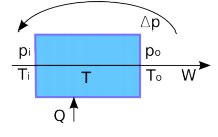
\includegraphics{img/tubo2.png}
\caption{Schema del tubo}
\label{fig:tubo2}
\end{figure}
Le equazioni idrauliche sono:
$$
\Delta p= \frac{K_T}{\rho}w^2-\rho g \Delta z
$$
Equazione di bilancio delle energie:
$$
\rho V c \dot{T_o}=cw(T_i-T_o)+Q
$$
\subsubsection{Pompe}
\begin{figure}[tbh]
\centering
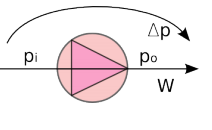
\includegraphics{img/pompa2.png}
\caption{Schema di una pompa}
\label{fig:pompa2}
\end{figure}
Esistono diversi tipi di pompe centrifughe o volumetriche, esse variano la loro portata in base alla loro velocit� comandata dal valore $n$. I flussi di massa e di volume sono proporzionali alla densit� $\rho$ e vengono indicati rispettivamente da $w$ e $q$.\\
Per quanto riguarda le pompe di tipo centrifugo:
$$
\Delta p= H0(n)-H1(n)w^2
$$
Mentre per quanto riguarda l'aspetto termico abbiamo che 
$$T_i=T_o$$
\subsubsection{Valvole}
\begin{figure}[tbh]
\centering
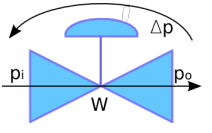
\includegraphics{img/valvola2.png}
\caption{Schema di una valvola}
\label{fig:valvola2}
\end{figure}
Le equazioni idrauliche e termiche sono rispettivamente:
$$
w=Cv_{max}\phi(x)\sqrt{\Delta p}
$$
$$T_i==T_o$$

\subsection{Scambi di calore}
\subsubsection{Scambio in un fluido}
\begin{figure}[tbh]
\centering
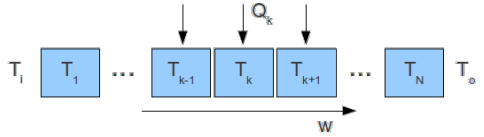
\includegraphics{img/flusso.png}
\caption{Scambio di calore in un fluido}
\label{fig:flusso}
\end{figure}
Per un fluido incomprimibile le equazioni di energia sono disaccoppiate da quelle idrauliche;dopo aver deciso la direzione del flusso le equazioni per ogni elemento sono descritte da:
$$\rho c V_k\dot{T_k}=wcT{k+1}-wcT_k+Q_k, \qquad T_{-1}=T_i, T_o=T_N$$
\subsubsection{Superfice metallica}
\begin{figure}[tbh]
\centering
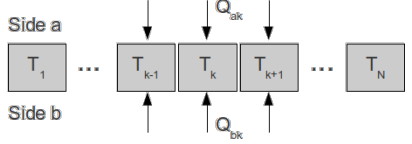
\includegraphics{img/metal2.png}
\caption{Scambio di calore con una superfice metallica}
\label{fig:metal2}
\end{figure}
Dividiamo il metallo nello stesso modo in cui abbiamo diviso il tubo in questo caso per� l'equazione diventa:
$$\rho_mc_mV_{mk}\dot{T_k}=Q_{ak}+Q_{bk}$$
\subsubsection{Scambio convettivo}
\begin{figure}[tbh]
\centering
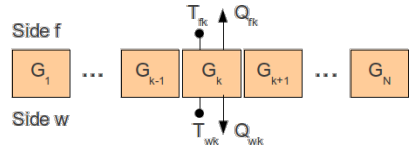
\includegraphics{img/convettivo2.png}
\caption{Scambio convettivo}
\label{fig:convettivo2}
\end{figure}
Per lo scambio convettivo adottiamo la stessa tecnica di discretizzazione perci� l'equazione di bilancio dell'energia diventa:
$$Q_{fk}=-Q_{wk}= \gamma S_k(T_{fk}-T_{wk})$$
dove il pedice "w" sta ad indicare il materiale di scambio e $S_k$ � la superfice di scambio.

\end{document}
